\chapter{Evaporation-conditioned embryo growth}
\label{ch:p9}

\begin{keybox}
\textbf{Key idea.} This is the whole story, at tutorial scale: a
\emph{wet} film \emph{dries} (Ch.~\ref{ch:p5}), the concentrating blend
\emph{phase-separates} (Ch.~\ref{ch:p1}--\ref{ch:p4}), and once the
crystallizable species is concentrated enough an \emph{implanted} crystal
embryo \emph{grows} (Ch.~\ref{ch:p6}) coupled back to composition
(Ch.~\ref{ch:p7}). The arc \emph{wet film $\to$ phase separation $\to$
embryo growth $\to$ crystalline film} is how a real solution-cast organic
solar cell forms.
\end{keybox}

\begin{keybox}
\textbf{Naming: embryo growth, not nucleation.} The default runs do
\emph{not} nucleate crystals from thermal noise --- they \emph{implant} a
supercritical embryo and ask whether the drying-conditioned local
composition lets it \emph{grow} or forces it to \emph{dissolve}. So this is
\emph{evaporation-conditioned embryo growth}. Genuine noise-driven
nucleation (Ch.~\ref{ch:p8}) is available as an advanced mode
(\code{make\_stepper(noise\_psi=...)}); it is slower and stochastic, so the
checked tutorial uses the deterministic implant.
\end{keybox}

\section{The solubility, derived from the free energy}

We run $(M,K)=(2,1)$ in film mode: a crystallizable small molecule
(species 0), a polymer (species 1), and an evaporating solvent. The r14
crystallization bulk carries a crystal-contact penalty $\chi_{ca}$. Compare
the homogeneous free energy at $\psi=1$ versus $\psi=0$ at fixed
composition: the $\psi$-dependent part changes by
%
\begin{equation}
  \Delta f = \phi_0\,\text{drive} + \phi_0\,\chi_{ca}\,(1-\phi_0),
  \qquad \text{drive}=\Delta h\,(T/T_m-1)<0,
\end{equation}
%
where the bulk drive lowers the crystal energy and the crystal-contact
penalty against the $(1-\phi_0)$ non-crystallizing surroundings raises it.
The crystal is favoured ($\Delta f<0$) iff
%
\begin{equation}
  \phi_0 > \phi^\star = 1 - \frac{|\text{drive}|}{\chi_{ca}}.
\end{equation}
%
This is a genuine \emph{solubility}: below the local small-molecule
fraction $\phi^\star$ an embryo redissolves; above it, it grows. For the
tutorial energetics ($\text{drive}=\ensuremath{\PnineDrive}$,
$\chi_{ca}=\ensuremath{\PnineChiCA}$) this gives the \emph{homogeneous}
solubility $\phi^\star=\ensuremath{\PninePhiStar}$.

\begin{keybox}
\textbf{Validated, with an honest caveat.} \code{embryo\_composition\_sweep}
implants the \emph{same} supercritical embryo into uniform blends of
increasing $\phi_0$ with \emph{no drying}, and brackets the grow/dissolve
crossover in
$[\ensuremath{\PnineCrossLo},\ensuremath{\PnineCrossHi}]$. The measured
crossover lies \emph{below} the derived $\phi^\star=\ensuremath{\PninePhiStar}$:
$\phi^\star$ is the \emph{homogeneous} solubility, but a supercritical
embryo \emph{enriches} $\phi_0$ in its neighbourhood as it orders (the
Chapter~\ref{ch:p7} crystal-bulk channel), lowering its effective growth
threshold. So the derivation is an \emph{upper bound}, and the sweep
confirms a composition threshold exists while lying below $\phi^\star$ ---
the honest, physically-grounded result.
\end{keybox}

\begin{keybox}
\textbf{Seeding is physical and delicate} (the S3b campaign lessons). The
implanted embryo radius $r_0$ must clear the Gibbs--Thomson critical radius
$r^\star$ with margin (sub-critical embryos redissolve), and the amplitude
must be near $1$. At a fixed super-solubility composition, a large embryo
($r_0=0.20$) grows but a small one ($r_0=0.05$) redissolves --- the
critical radius, not just the composition. We read the \emph{terminal}
crystalline state, not a mid-growth snapshot.
\end{keybox}

\section{The arc: wet dissolves, dry grows}

Drying \emph{raises} the local $\phi_0$, so the \emph{same} embryo behaves
oppositely depending on \emph{when} it is introduced:
\begin{itemize}[nosep]
  \item implanted in the \textbf{wet} film ($\phi_s=\ensuremath{\PnineWetPhis}$,
        local $\phi_0$ below $\phi^\star$) it \emph{dissolves}
        (terminal area $\ensuremath{\PnineWetEnd}$,
        $\psi_{\max}=\ensuremath{\PnineWetPsimax}$);
  \item implanted \textbf{mid-drying} ($\phi_s=\ensuremath{\PnineDryPhis}$,
        $\phi_0$ above $\phi^\star$) it \emph{grows} to a crystalline film
        (terminal area $\ensuremath{\PnineDryEnd}$,
        $\psi_{\max}=\ensuremath{\PnineDryPsimax}$).
\end{itemize}
The fate is set by the drying-\emph{conditioned local composition} relative
to $\phi^\star$ --- not by time or evaporation \emph{per se}, which is
exactly what the no-drying composition sweep isolates.

\begin{keybox}
\textbf{Termination, honestly.} A march that stops at the requested time
horizon is a \code{time\_horizon} stop --- \emph{not} a ``drying time''. The
honest status enum is \code{time\_horizon} / \code{solvent\_target}
(dryness) / \code{height\_floor} / \code{min\_dt} (Newton/stiffness) /
\code{step\_budget}; the wet and dry legs terminate
\code{[\PnineWetTerm]} and \code{[\PnineDryTerm]}.
\textbf{Recorded simplification:} constant Onsager mobility with cuDSS
instead of the production Vignes composition-singular mobility
(\file{tests/test\_multiphase\_s3.py}); the qualitative arc is unchanged,
the drying-front sharpness softened.
\end{keybox}

\section{Run it}

\begin{runbox}
\textbf{Run it.}
\begin{lstlisting}
cd physics/09_evaporation_crystallization
python run.py            # solubility + controls + arc + checks
\end{lstlisting}
It derives $\phi^\star$, validates it by the composition sweep, runs the
sub/supercritical embryo control and the wet-vs-dry arc, and checks
\file{outputs/results.json} against \file{baseline.yaml}. Compare with
\file{EXPECTED.md} and the figures.
\end{runbox}

% --- generated by gen_figures.py ---
\begin{figure}[h]\centering
  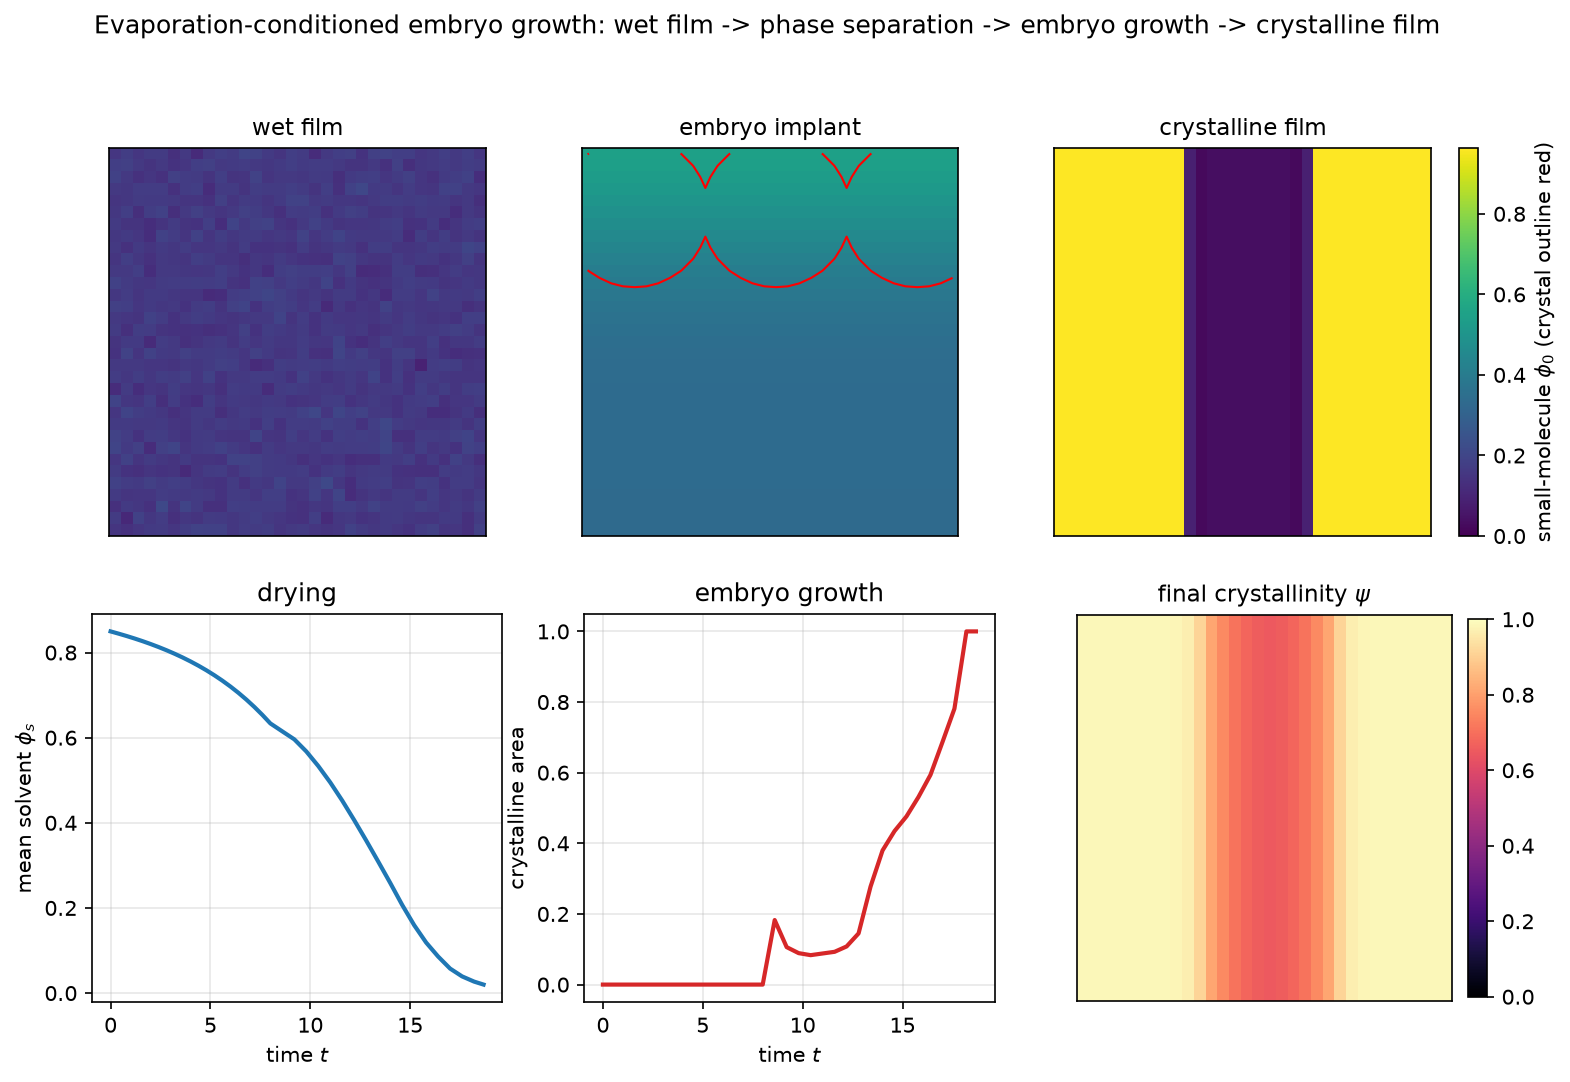
\includegraphics[width=\linewidth]{figures/p9_arc.png}
  \caption{The arc (dry-implant run): top --- wet film, embryo implant, and
    the final crystalline film ($\phi_0$ with crystal outline in red);
    bottom --- the drying curve $\phi_s(t)$, the crystalline-area growth,
    and the final crystallinity $\psi$.}
  \label{fig:p9arc}
\end{figure}

\begin{figure}[h]\centering
  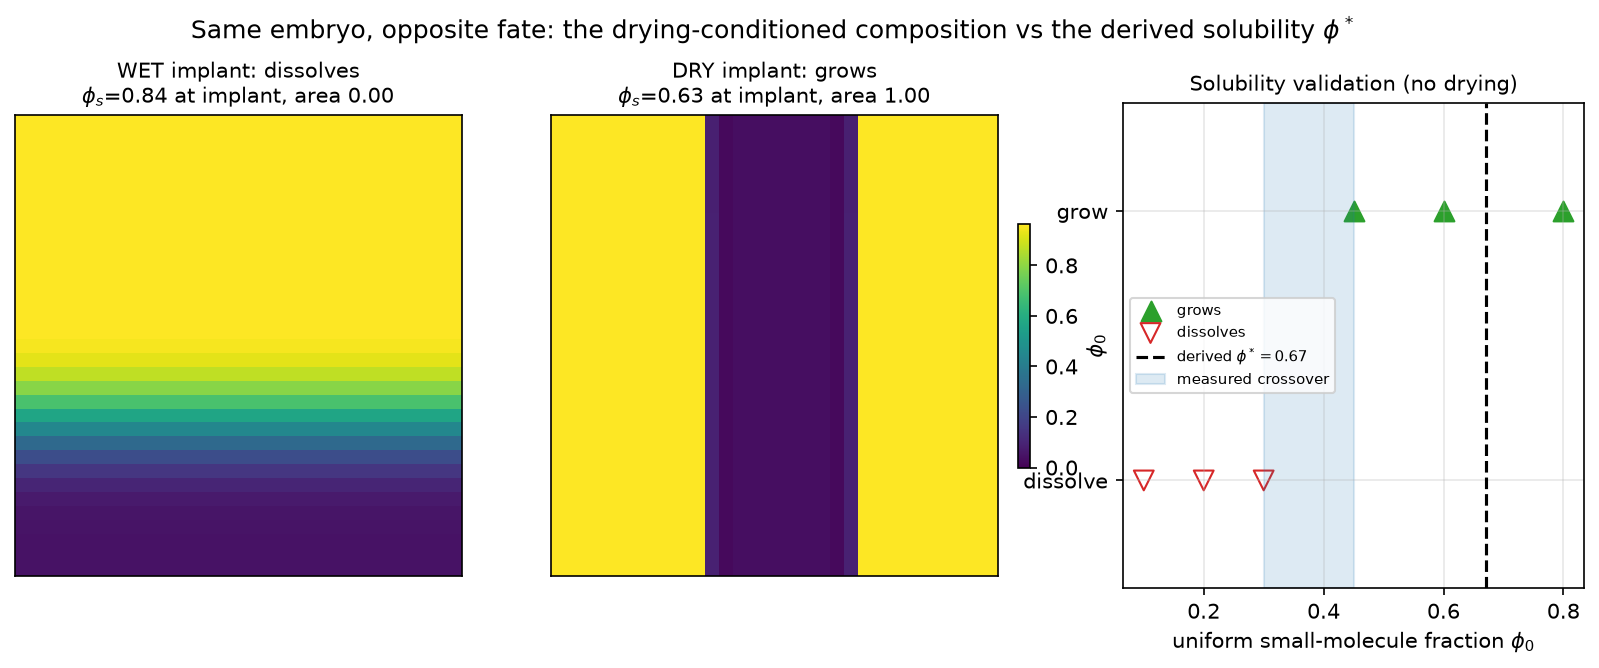
\includegraphics[width=\linewidth]{figures/p9_wet_vs_dry.png}
  \caption{Left/middle: the same embryo, implanted wet (dissolves) vs
    mid-drying (grows). Right: the solubility validation --- implanting into
    uniform blends of varying $\phi_0$ (no drying) brackets the derived
    $\phi^\star$.}
  \label{fig:p9wetdry}
\end{figure}

\begin{keybox}
\textbf{Measured self-check} (level 5, cuDSS; tolerance-checked in
\file{baseline.yaml}).
\begin{center}\small
\begin{tabular}{lcc}
\toprule
 & wet implant & dry implant \\
\midrule
$\phi_s$ at implant       & \ensuremath{\PnineWetPhis} & \ensuremath{\PnineDryPhis} \\
crystalline area (terminal) & \ensuremath{\PnineWetEnd} & \ensuremath{\PnineDryEnd} \\
$\psi_{\max}$ (terminal)  & \ensuremath{\PnineWetPsimax} & \ensuremath{\PnineDryPsimax} \\
\bottomrule
\end{tabular}\\[4pt]
derived $\phi^\star=\ensuremath{\PninePhiStar}$; measured crossover
$[\ensuremath{\PnineCrossLo},\ensuremath{\PnineCrossHi}]$.
\end{center}
\end{keybox}

\section{Code walk-through}

\paragraph{1. The derived solubility.} \code{solubility\_threshold} returns
$\phi^\star=1-|\text{drive}|/\chi_{ca}$ from the r14 free energy;
\code{embryo\_composition\_sweep} validates it with no-drying static-blend
implants.

\paragraph{2. The drying, crystallizing film.} \code{make\_stepper} builds
the $(2,1)$ film-mode stepper (r14, cuDSS) and asserts the crystal
energetics reached it --- the missing-splat guard from the S3b campaign
(a dropped keyword silently defaulted $T_m=1$, a huge \emph{melting} force).

\paragraph{3. Implant, march, read the terminal state.} \code{run\_arc}
marches the drying film to the implant time, calls \code{implant}, marches
on, and reports the terminal area, $\psi_{\max}$ and the honest termination
status.

\section{Explore on your own}

\question{Sweep the implant time from wet to dry. Is there a sharp
crossover in $\phi_s$ between dissolution and growth, and does the LOCAL
$\phi_0$ at that crossover match the derived $\phi^\star$?}

\question{Vary $\chi_{ca}$ and re-derive $\phi^\star$. Re-run the
composition sweep --- does the measured crossover track
$1-|\text{drive}|/\chi_{ca}$? Where does $\phi^\star$ hit $0$ (no
solubility barrier: the embryo grows even wet)?}

\question{Vary the implant radius $r_0$ around the critical radius at a
super-solubility composition. Find the margin below which even a
mid-drying embryo redissolves --- the Gibbs--Thomson $r^\star$.}

\question{Switch on the advanced FDT-noise mode
(\code{make\_stepper(noise\_psi=...)}) and let the drying film nucleate on
its own. Does crystallization still wait for the solvent to leave? What
sets the number of crystals?}

\question{This is the design problem: given a target (fine, pure,
bicontinuous crystalline domains), which knobs --- $k_e$, $\chi_{ca}$,
undercooling, blend ratio --- would you turn, and which fight each other?
(The Differentiable track answers this with gradients.)}

% ====================================================================
